\documentclass[12pt,fleqn]{article}\usepackage{../../common}
\begin{document}
Ders 26

[giriş bölümü atlandı]

Dersin son 10 dakikasında iki boyutlu sonlu öğeler (finite elements -FEM-)
konusuna giriş yapalım. Problem alanını temsil etmek için üçgenler kullanacağım,
izgara üçgen bazlı yani. Kareler vs de olabilirdi..

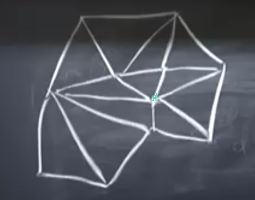
\includegraphics[width=20em]{compscieng_1_26_01.png}

Önemli nokta şu, üçgenler gelişigüzel noktalarda olabilir, düğümlerin nerede,
üçgenlerin ne şekillerde olacağını biz belirleriz. Bu FEM yaklaşımının güçlü
taraflarından biri. Üstteki izgara fena değil, 180 açıli üçgenler yok (o zaman
öteki açılar yamyassı hale gelirdi, üçgen ise yaramazdı). Tabii yapısız dahi
olsa izgarayı yaratmak için bir program kullanmak iyi olur, benim bir
tez öğrencim böyle bir programı geçende yazdı [hoca bugünlerde pek çok kişinin
kullandığı \verb!dıştmesh! programından [1] bahsediyor herhalde]. 
















Kaynaklar

[1] DistMesh, \url{http://persson.berkeley.edu/distmesh/}

\end{document}
